\documentclass{article}
\usepackage{graphicx}
% Custom definitions
% To use this customization file, insert the line "% Custom definitions
% To use this customization file, insert the line "% Custom definitions
% To use this customization file, insert the line "\input{custom}" in the header of the tex file.

% Formatting

\tolerance=1000
\usepackage[margin=1in]{geometry}


% Packages

% \usepackage{amssymb,latexsym}
\usepackage{amssymb,amsfonts,amsmath,latexsym,amsthm}
%\usepackage[usenames,dvipsnames]{color}
\usepackage[]{graphicx}
\usepackage[space]{grffile}
\usepackage{mathrsfs}   % fancy math font
% \usepackage[font=small,skip=0pt]{caption}
\usepackage[skip=0pt]{caption}
\usepackage{subcaption}
\usepackage{verbatim}
\usepackage{url}
\usepackage{bm}
\usepackage{dsfont}
\usepackage{extarrows}
\usepackage{multirow}
% \usepackage{wrapfig}
% \usepackage{epstopdf}
\usepackage{rotating}
\usepackage{tikz}
\usetikzlibrary{fit}					% fitting shapes to coordinates
%\usetikzlibrary{backgrounds}	% drawing the background after the foreground


% \usepackage[dvipdfm,colorlinks,citecolor=blue,linkcolor=blue,urlcolor=blue]{hyperref}
\usepackage[colorlinks,citecolor=blue,linkcolor=blue,urlcolor=blue]{hyperref}
%\usepackage{hyperref}
\usepackage[authoryear,round]{natbib}


%  Theorems, etc.

\theoremstyle{plain}
\newtheorem{theorem}{Theorem}[section]
\newtheorem{corollary}[theorem]{Corollary}
\newtheorem{lemma}[theorem]{Lemma}
\newtheorem{proposition}[theorem]{Proposition}
\newtheorem{condition}[theorem]{Condition}
% \newtheorem{conditions}[theorem]{Conditions}

\theoremstyle{definition}
\newtheorem{definition}[theorem]{Definition}
% \newtheorem*{unnumbered-definition}{Definition}
\newtheorem{example}[theorem]{Example}
\theoremstyle{remark}
\newtheorem*{remark}{Remark}
\numberwithin{equation}{section}




% Document-specific shortcuts
\newcommand{\btheta}{{\bm\theta}}
\newcommand{\bbtheta}{{\pmb{\bm\theta}}}

\newcommand{\commentary}[1]{\ifx\showcommentary\undefined\else \emph{#1}\fi}

\newcommand{\term}[1]{\textit{\textbf{#1}}}

% Math shortcuts

% Probability distributions
\DeclareMathOperator*{\Exp}{Exp}
\DeclareMathOperator*{\TExp}{TExp}
\DeclareMathOperator*{\Bernoulli}{Bernoulli}
\DeclareMathOperator*{\Beta}{Beta}
\DeclareMathOperator*{\Ga}{Gamma}
\DeclareMathOperator*{\TGamma}{TGamma}
\DeclareMathOperator*{\Poisson}{Poisson}
\DeclareMathOperator*{\Binomial}{Binomial}
\DeclareMathOperator*{\NormalGamma}{NormalGamma}
\DeclareMathOperator*{\InvGamma}{InvGamma}
\DeclareMathOperator*{\Cauchy}{Cauchy}
\DeclareMathOperator*{\Uniform}{Uniform}
\DeclareMathOperator*{\Gumbel}{Gumbel}
\DeclareMathOperator*{\Pareto}{Pareto}
\DeclareMathOperator*{\Mono}{Mono}
\DeclareMathOperator*{\Geometric}{Geometric}
\DeclareMathOperator*{\Wishart}{Wishart}

% Math operators
\DeclareMathOperator*{\argmin}{arg\,min}
\DeclareMathOperator*{\argmax}{arg\,max}
\DeclareMathOperator*{\Cov}{Cov}
\DeclareMathOperator*{\diag}{diag}
\DeclareMathOperator*{\median}{median}
\DeclareMathOperator*{\Vol}{Vol}

% Math characters
\newcommand{\R}{\mathbb{R}}
\newcommand{\Z}{\mathbb{Z}}
\newcommand{\E}{\mathbb{E}}
\renewcommand{\Pr}{\mathbb{P}}
\newcommand{\I}{\mathds{1}}
\newcommand{\V}{\mathbb{V}}

\newcommand{\A}{\mathcal{A}}
\newcommand{\C}{\mathcal{C}}
\newcommand{\D}{\mathcal{D}}
\newcommand{\Hcal}{\mathcal{H}}
\newcommand{\M}{\mathcal{M}}
\newcommand{\N}{\mathcal{N}}
\newcommand{\X}{\mathcal{X}}
\newcommand{\Zcal}{\mathcal{Z}}
\renewcommand{\P}{\mathcal{P}}

\newcommand{\T}{\mathtt{T}}
\renewcommand{\emptyset}{\varnothing}


% Miscellaneous commands
\newcommand{\iid}{\stackrel{\mathrm{iid}}{\sim}}
\newcommand{\matrixsmall}[1]{\bigl(\begin{smallmatrix}#1\end{smallmatrix} \bigr)}

\newcommand{\items}[1]{\begin{itemize} #1 \end{itemize}}

\newcommand{\todo}[1]{\emph{\textcolor{red}{(#1)}}}

\newcommand{\branch}[4]{
\left\{
	\begin{array}{ll}
		#1  & \mbox{if } #2 \\
		#3 & \mbox{if } #4
	\end{array}
\right.
}

% approximately proportional to
\def\app#1#2{%
  \mathrel{%
    \setbox0=\hbox{$#1\sim$}%
    \setbox2=\hbox{%
      \rlap{\hbox{$#1\propto$}}%
      \lower1.3\ht0\box0%
    }%
    \raise0.25\ht2\box2%
  }%
}
\def\approxprop{\mathpalette\app\relax}

% \newcommand{\approptoinn}[2]{\mathrel{\vcenter{
  % \offinterlineskip\halign{\hfil$##$\cr
    % #1\propto\cr\noalign{\kern2pt}#1\sim\cr\noalign{\kern-2pt}}}}}

% \newcommand{\approxpropto}{\mathpalette\approptoinn\relax}





" in the header of the tex file.

% Formatting

\tolerance=1000
\usepackage[margin=1in]{geometry}


% Packages

% \usepackage{amssymb,latexsym}
\usepackage{amssymb,amsfonts,amsmath,latexsym,amsthm}
%\usepackage[usenames,dvipsnames]{color}
\usepackage[]{graphicx}
\usepackage[space]{grffile}
\usepackage{mathrsfs}   % fancy math font
% \usepackage[font=small,skip=0pt]{caption}
\usepackage[skip=0pt]{caption}
\usepackage{subcaption}
\usepackage{verbatim}
\usepackage{url}
\usepackage{bm}
\usepackage{dsfont}
\usepackage{extarrows}
\usepackage{multirow}
% \usepackage{wrapfig}
% \usepackage{epstopdf}
\usepackage{rotating}
\usepackage{tikz}
\usetikzlibrary{fit}					% fitting shapes to coordinates
%\usetikzlibrary{backgrounds}	% drawing the background after the foreground


% \usepackage[dvipdfm,colorlinks,citecolor=blue,linkcolor=blue,urlcolor=blue]{hyperref}
\usepackage[colorlinks,citecolor=blue,linkcolor=blue,urlcolor=blue]{hyperref}
%\usepackage{hyperref}
\usepackage[authoryear,round]{natbib}


%  Theorems, etc.

\theoremstyle{plain}
\newtheorem{theorem}{Theorem}[section]
\newtheorem{corollary}[theorem]{Corollary}
\newtheorem{lemma}[theorem]{Lemma}
\newtheorem{proposition}[theorem]{Proposition}
\newtheorem{condition}[theorem]{Condition}
% \newtheorem{conditions}[theorem]{Conditions}

\theoremstyle{definition}
\newtheorem{definition}[theorem]{Definition}
% \newtheorem*{unnumbered-definition}{Definition}
\newtheorem{example}[theorem]{Example}
\theoremstyle{remark}
\newtheorem*{remark}{Remark}
\numberwithin{equation}{section}




% Document-specific shortcuts
\newcommand{\btheta}{{\bm\theta}}
\newcommand{\bbtheta}{{\pmb{\bm\theta}}}

\newcommand{\commentary}[1]{\ifx\showcommentary\undefined\else \emph{#1}\fi}

\newcommand{\term}[1]{\textit{\textbf{#1}}}

% Math shortcuts

% Probability distributions
\DeclareMathOperator*{\Exp}{Exp}
\DeclareMathOperator*{\TExp}{TExp}
\DeclareMathOperator*{\Bernoulli}{Bernoulli}
\DeclareMathOperator*{\Beta}{Beta}
\DeclareMathOperator*{\Ga}{Gamma}
\DeclareMathOperator*{\TGamma}{TGamma}
\DeclareMathOperator*{\Poisson}{Poisson}
\DeclareMathOperator*{\Binomial}{Binomial}
\DeclareMathOperator*{\NormalGamma}{NormalGamma}
\DeclareMathOperator*{\InvGamma}{InvGamma}
\DeclareMathOperator*{\Cauchy}{Cauchy}
\DeclareMathOperator*{\Uniform}{Uniform}
\DeclareMathOperator*{\Gumbel}{Gumbel}
\DeclareMathOperator*{\Pareto}{Pareto}
\DeclareMathOperator*{\Mono}{Mono}
\DeclareMathOperator*{\Geometric}{Geometric}
\DeclareMathOperator*{\Wishart}{Wishart}

% Math operators
\DeclareMathOperator*{\argmin}{arg\,min}
\DeclareMathOperator*{\argmax}{arg\,max}
\DeclareMathOperator*{\Cov}{Cov}
\DeclareMathOperator*{\diag}{diag}
\DeclareMathOperator*{\median}{median}
\DeclareMathOperator*{\Vol}{Vol}

% Math characters
\newcommand{\R}{\mathbb{R}}
\newcommand{\Z}{\mathbb{Z}}
\newcommand{\E}{\mathbb{E}}
\renewcommand{\Pr}{\mathbb{P}}
\newcommand{\I}{\mathds{1}}
\newcommand{\V}{\mathbb{V}}

\newcommand{\A}{\mathcal{A}}
\newcommand{\C}{\mathcal{C}}
\newcommand{\D}{\mathcal{D}}
\newcommand{\Hcal}{\mathcal{H}}
\newcommand{\M}{\mathcal{M}}
\newcommand{\N}{\mathcal{N}}
\newcommand{\X}{\mathcal{X}}
\newcommand{\Zcal}{\mathcal{Z}}
\renewcommand{\P}{\mathcal{P}}

\newcommand{\T}{\mathtt{T}}
\renewcommand{\emptyset}{\varnothing}


% Miscellaneous commands
\newcommand{\iid}{\stackrel{\mathrm{iid}}{\sim}}
\newcommand{\matrixsmall}[1]{\bigl(\begin{smallmatrix}#1\end{smallmatrix} \bigr)}

\newcommand{\items}[1]{\begin{itemize} #1 \end{itemize}}

\newcommand{\todo}[1]{\emph{\textcolor{red}{(#1)}}}

\newcommand{\branch}[4]{
\left\{
	\begin{array}{ll}
		#1  & \mbox{if } #2 \\
		#3 & \mbox{if } #4
	\end{array}
\right.
}

% approximately proportional to
\def\app#1#2{%
  \mathrel{%
    \setbox0=\hbox{$#1\sim$}%
    \setbox2=\hbox{%
      \rlap{\hbox{$#1\propto$}}%
      \lower1.3\ht0\box0%
    }%
    \raise0.25\ht2\box2%
  }%
}
\def\approxprop{\mathpalette\app\relax}

% \newcommand{\approptoinn}[2]{\mathrel{\vcenter{
  % \offinterlineskip\halign{\hfil$##$\cr
    % #1\propto\cr\noalign{\kern2pt}#1\sim\cr\noalign{\kern-2pt}}}}}

% \newcommand{\approxpropto}{\mathpalette\approptoinn\relax}





" in the header of the tex file.

% Formatting




% Packages

\setbeamertemplate{navigation symbols}{}
\setbeamertemplate{footline}[page number]

 \usepackage{amssymb,latexsym}
\usepackage{amssymb,amsfonts,amsmath,latexsym,amsthm, bm}
%\usepackage[usenames,dvipsnames]{color}
%\usepackage[]{graphicx}
%\usepackage[space]{grffile}
\usepackage{mathrsfs}   % fancy math font
% \usepackage[font=small,skip=0pt]{caption}
%\usepackage[skip=0pt]{caption}
%\usepackage{subcaption}
%\usepackage{verbatim}
%\usepackage{url}
%\usepackage{bm}
\usepackage{dsfont}
\usepackage{multirow}
%\usepackage{extarrows}
%\usepackage{multirow}
%% \usepackage{wrapfig}
%% \usepackage{epstopdf}
%\usepackage{rotating}
%\usepackage{tikz}
%\usetikzlibrary{fit}					% fitting shapes to coordinates
%\usetikzlibrary{backgrounds}	% drawing the background after the foreground


% \usepackage[dvipdfm,colorlinks,citecolor=blue,linkcolor=blue,urlcolor=blue]{hyperref}
%\usepackage[colorlinks,citecolor=blue,linkcolor=blue,urlcolor=blue]{hyperref}
%%\usepackage{hyperref}
%\usepackage[authoryear,round]{natbib}


%  Theorems, etc.

%\theoremstyle{plain}
%\newtheorem{theorem}{Theorem}[section]
%\newtheorem{corollary}[theorem]{Corollary}
%\newtheorem{lemma}[theorem]{Lemma}
%\newtheorem{proposition}[theorem]{Proposition}
%\newtheorem{condition}[theorem]{Condition}
% \newtheorem{conditions}[theorem]{Conditions}

%\theoremstyle{definition}
%\newtheorem{definition}[theorem]{Definition}
%% \newtheorem*{unnumbered-definition}{Definition}
%\newtheorem{example}[theorem]{Example}
%\theoremstyle{remark}
%\newtheorem*{remark}{Remark}
%\numberwithin{equation}{section}




% Document-specific shortcuts
\newcommand{\btheta}{{\bm\theta}}
\newcommand{\bbtheta}{{\pmb{\bm\theta}}}

\newcommand{\commentary}[1]{\ifx\showcommentary\undefined\else \emph{#1}\fi}

\newcommand{\term}[1]{\textit{\textbf{#1}}}

% Math shortcuts

% Probability distributions
\DeclareMathOperator*{\Exp}{Exp}
\DeclareMathOperator*{\TExp}{TExp}
\DeclareMathOperator*{\Bernoulli}{Bernoulli}
\DeclareMathOperator*{\Beta}{Beta}
\DeclareMathOperator*{\Ga}{Gamma}
\DeclareMathOperator*{\TGamma}{TGamma}
\DeclareMathOperator*{\Poisson}{Poisson}
\DeclareMathOperator*{\Binomial}{Binomial}
\DeclareMathOperator*{\NormalGamma}{NormalGamma}
\DeclareMathOperator*{\InvGamma}{InvGamma}
\DeclareMathOperator*{\Cauchy}{Cauchy}
\DeclareMathOperator*{\Uniform}{Uniform}
\DeclareMathOperator*{\Gumbel}{Gumbel}
\DeclareMathOperator*{\Pareto}{Pareto}
\DeclareMathOperator*{\Mono}{Mono}
\DeclareMathOperator*{\Geometric}{Geometric}
\DeclareMathOperator*{\Wishart}{Wishart}

% Math operators
\DeclareMathOperator*{\argmin}{arg\,min}
\DeclareMathOperator*{\argmax}{arg\,max}
\DeclareMathOperator*{\Cov}{Cov}
\DeclareMathOperator*{\diag}{diag}
\DeclareMathOperator*{\median}{median}
\DeclareMathOperator*{\Vol}{Vol}

% Math characters
\newcommand{\R}{\mathbb{R}}
\newcommand{\Z}{\mathbb{Z}}
\newcommand{\E}{\mathbb{E}}
\renewcommand{\Pr}{\mathbb{P}}
\newcommand{\I}{\mathds{1}}
\newcommand{\V}{\mathbb{V}}

\newcommand{\A}{\mathcal{A}}
%\newcommand{\C}{\mathcal{C}}
\newcommand{\D}{\mathcal{D}}
\newcommand{\Hcal}{\mathcal{H}}
\newcommand{\M}{\mathcal{M}}
\newcommand{\N}{\mathcal{N}}
\newcommand{\X}{\mathcal{X}}
\newcommand{\Zcal}{\mathcal{Z}}
\renewcommand{\P}{\mathcal{P}}

\newcommand{\T}{\mathtt{T}}
\renewcommand{\emptyset}{\varnothing}


% Miscellaneous commands
\newcommand{\iid}{\stackrel{\mathrm{iid}}{\sim}}
\newcommand{\matrixsmall}[1]{\bigl(\begin{smallmatrix}#1\end{smallmatrix} \bigr)}

\newcommand{\items}[1]{\begin{itemize} #1 \end{itemize}}

\newcommand{\todo}[1]{\emph{\textcolor{red}{(#1)}}}

\newcommand{\branch}[4]{
\left\{
	\begin{array}{ll}
		#1  & \mbox{if } #2 \\
		#3 & \mbox{if } #4
	\end{array}
\right.
}

% approximately proportional to
\def\app#1#2{%
  \mathrel{%
    \setbox0=\hbox{$#1\sim$}%
    \setbox2=\hbox{%
      \rlap{\hbox{$#1\propto$}}%
      \lower1.3\ht0\box0%
    }%
    \raise0.25\ht2\box2%
  }%
}
\def\approxprop{\mathpalette\app\relax}

% \newcommand{\approptoinn}[2]{\mathrel{\vcenter{
  % \offinterlineskip\halign{\hfil$##$\cr
    % #1\propto\cr\noalign{\kern2pt}#1\sim\cr\noalign{\kern-2pt}}}}}

% \newcommand{\approxpropto}{\mathpalette\approptoinn\relax}







\begin{document}

\title{Lab 4: Bayesian Statistics in \textsf{R} - STA 360/602}
\author{Rebecca C. Steorts}
\date{}
\maketitle

%\section{Agenda}
%\begin{enumerate}
%%\item{Common errors from Lab 6}
%\item{Importance of writing well and documenting code well}
%\item{Using \textsf{dbeta}}
%\item{Using \textsf{rbeta}}
%\item{Generating a sequence using \textsf{seq}}
%\item{Plotting multiple items in the same window using \textsf{plot}}
%\end{enumerate}

\section{Agenda}
Do a teacher's expectations influence student achievement? In a famous study, Rosenthal and Jacobson (1968) performed an experiment in a California elementary school to try to answer this question. At the beginning of the year, all students were given an IQ test.  For each class, the researchers randomly selected around 20\% of the students, and told the teacher that these students were ``spurters'' that could be expected to perform particularly well that year. (This was not based on the test---the spurters were randomly chosen.) At the end of the year, all students were given another IQ test. The change in IQ score for the first-grade students was:\footnote{The original data is not available. This data is from the \texttt{ex1321} dataset of the \texttt{R} package \texttt{Sleuth3}, which was constructed to match the summary statistics and conclusions of the original study.}

\begin{quote}
spurters (S)\\
$x$ = (18, 40, 15, 17, 20, 44, 38)
\end{quote}
\begin{quote}
controls (C)\\
$y$ = (--4, 0, --19, 24, 19, 10, 5, 10, 29, 13, --9, --8, 20, --1, 12, 21, --7, 14,
     13, 20, 11, 16, 15, 27, 23, 36, --33, 34, 13, 11, --19, 21, 6, 25, 30,
     22, --28, 15, 26, --1, --2, 43, 23, 22, 25, 16, 10, 29)
\end{quote}




\begin{enumerate}
\item Plot histograms for the change in IQ score for the two groups. Report your findings. 
\item How strongly does this data support the hypothesis that the teachers? expectations caused the spurters to perform better than their classmates? 
IQ tests are purposefully calibrated to make the scores normally distributed, so it makes sense to use a normal model here:
\begin{align*}
\text{spurters: } X_1,\dotsc,X_{n_S}\iid \N(\mu_S,\lambda_S^{-1})\\
\text{controls: } Y_1,\dotsc,Y_{n_C}\iid \N(\mu_C,\lambda_C^{-1}).
\end{align*}
We are interested in the difference between the means---in particular, is $\mu_S>\mu_C$?
We don't know the standard deviations $\sigma_S=\lambda_S^{-1/2}$ and $\sigma_C=\lambda_C^{-1/2}$, and the sample seems too small to estimate them very well.

it is easy using a Bayesian approach: we just need to compute the posterior probability that $\mu_S>\mu_C$:
$$ \Pr(\bm\mu_S > \bm\mu_C \mid x_{1:n_S},y_{1:n_C}). $$

Let's use independent NormalGamma priors:
\begin{align*}
\text{spurters: } (\bm\mu_S,\bm\lambda_S) \sim \NormalGamma(m,c,a,b)\\
\text{controls: } (\bm\mu_C,\bm\lambda_C) \sim \NormalGamma(m,c,a,b)
\end{align*}

with the following hyperparameter settings, based on subjective prior knowledge:
\begin{itemize}
\item $m = 0$ (Don't know whether students will improve or not, on average.)
\item $c = 1$ (Unsure about how big the mean change will be---prior certainty in our choice of $m$ assessed to be equivalent to one datapoint.)
\item $a = 1/2$ (Unsure about how big the standard deviation of the changes will be.)
\item $b = 10^2 a$ (Standard deviation of the changes expected to be around $10 = \sqrt{b/a} = \E(\lambda)^{-1/2}$.)
\end{itemize}

The updated posterior parameters are
\begin{align*}
\text{for spurters:} & \\
    M & =\frac{1\cdot 0 + 7 \cdot 27.43}{1 + 7} = 24.0\\
    C & = 1 + 7 = 8\\
    A & = 1/2 + 7/2 = 4\\ 
    B &= 100/2 + \tfrac{1}{2}\cdot 7\cdot 11.66^2 + \tfrac{1}{2}\frac{1\cdot 7}{1 + 7}(27.43 - 0)^2 = 855.0 \\
\text{for controls:} & \\
    M & =\frac{1\cdot 0 + 48\cdot 12.04}{1 + 48} = 11.8\\
    C & = 1 + 48 = 49\\
    A & = 1/2 + 48/2 = 24.5\\
    B &= 100/2 + \tfrac{1}{2}\cdot 48\cdot 16.10^2 + \tfrac{1}{2}\frac{1\cdot 48}{1 + 48}(12.04 - 0)^2 = 6344.0
\end{align*}

which implies that 

\begin{align*}
\bm\mu_S,\bm\lambda_S\mid x_{1:n_S} &\,\sim\,\NormalGamma(24.0,8,4,855.0)\\
\bm\mu_C,\bm\lambda_C\mid y_{1:n_C} &\,\sim\,\NormalGamma(11.8,49,24.5,6344.0).
\end{align*}

\item Based on the calculations from the previous task, provide a scatterplot of samples from the posterior distributions for the two groups. Your scatterplot should look similar to Figure \ref{figure:pygmalion-posteriors}. What are your conclusions? 


\begin{figure}
  \begin{center}
    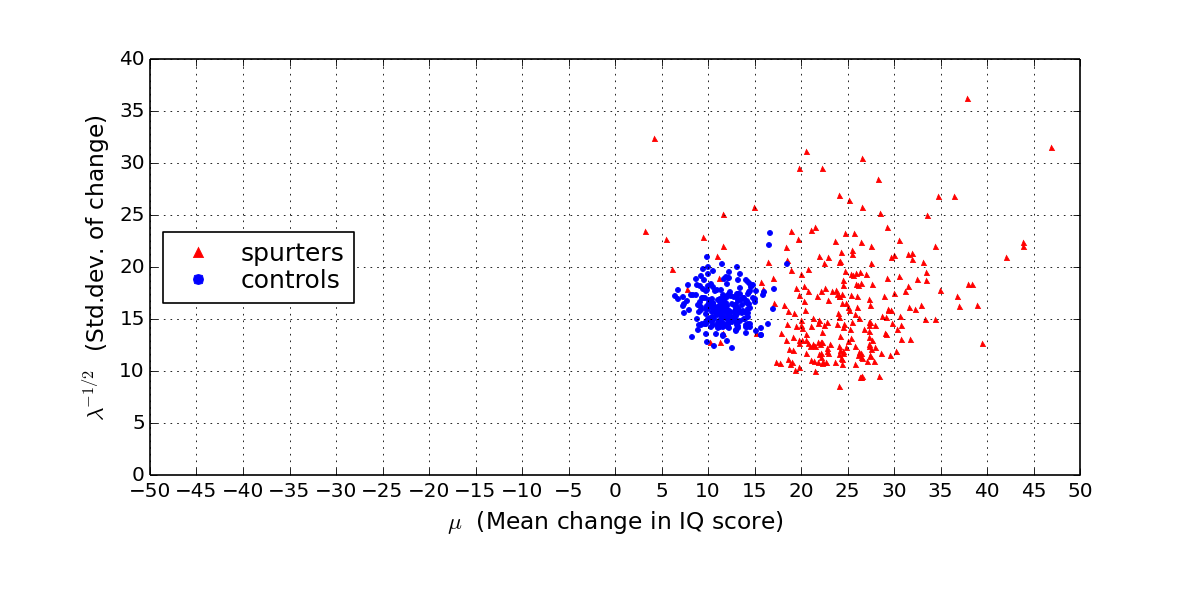
\includegraphics[width=1\textwidth]{examples/pygmalion-posteriors.png}
    % Source: Original work by J. W. Miller.
  \end{center}
  \caption{Samples of $(\mu,\sigma)$ from the posteriors for the two groups.}
  \label{figure:pygmalion-posteriors}
\end{figure}


\item Now, we can answer our original question: ``What is the posterior probability that $\mu_S>\mu_C$?'' \\

The easiest way to do this is to take a bunch of samples from each of the posteriors, and see what fraction of times we have $\mu_S>\mu_C$. This is an example of a Monte Carlo approximation (much more to come on this in the future). 

To do this, we draw $N=10^6$ samples from each posterior:
\begin{align*}
&(\mu_S^{(1)},\lambda_S^{(1)}),\dotsc,(\mu_S^{(N)},\lambda_S^{(N)})\sim \NormalGamma(24.0,8,4,855.0)\\
&(\mu_C^{(1)},\lambda_C^{(1)}),\dotsc,(\mu_C^{(N)},\lambda_C^{(N)})\sim\NormalGamma(11.8,49,24.5,6344.0)
\end{align*}
and obtain the approximation
\begin{align*}
\Pr(\bm\mu_S > \bm\mu_C \mid x_{1:n_S},y_{1:n_C}) 
\approx \frac{1}{N} \sum_{i = 1}^N \I\big(\mu_S^{(i)}>\mu_C^{(i)}\big) =  \;\;??
\end{align*}

Interpret the posterior probability that you compute above. 

\item Let's return back to the prior assumptions. There are a few ways that you can check that the prior conforms with our prior beliefs. Let's go back and checks these. Draw some samples from the prior and look at them---this is probably the best general strategy. See Figure \ref{figure:pygmalion-prior}. It's also a good idea to look at sample hypothetical datasets $X_{1:n}$ drawn using these sampled parameter values. 

Please replicate a plot similar to Figure \ref{figure:pygmalion-prior} and report your findings. 

\begin{figure}
  \begin{center}
    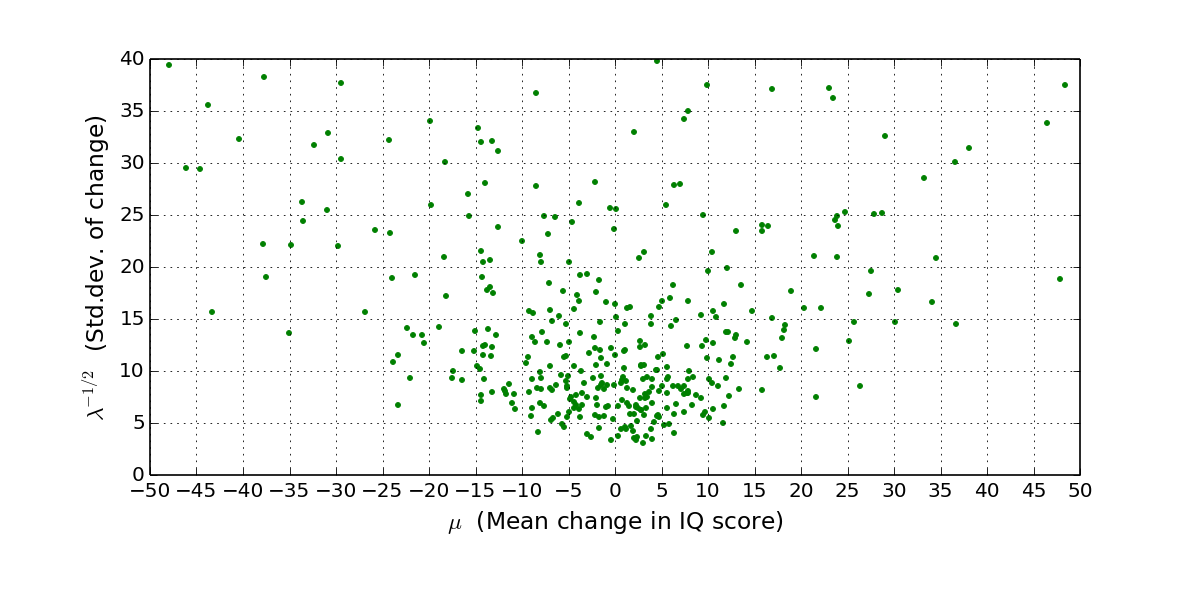
\includegraphics[width=1\textwidth]{examples/pygmalion-prior.png}
    % Source: Original work by J. W. Miller.
  \end{center}
  \caption{Samples of $(\mu,\sigma)$ from the prior.}
  \label{figure:pygmalion-prior}
\end{figure}




\end{enumerate}

%\section{Directions}
%
%In general for Labs, at the top of any file you are asked to submit, please list the following:
%
%\begin{enumerate}
%\item{First Name Last Name}
%\item{Lab Date}
%\item{Team Member(s)}
%\end{enumerate}
%
%\noindent
%With respect to any item for which you are asked to generate any output, please provide the actual \textsf{R} output as a part of your solution and any explanation needed as well. For any functions/ computations that you will write, please list the following as comments before the step in \textsf{R}:
%
%\begin{enumerate}
%\item{Task number and descriptions.}
%\item{Input(s) with descriptions.}
%\item{Outputs(s) with descriptions.}
%\item{Function/ output summary (along with intermediate step comments).}
%\end{enumerate} 
%
%\noindent
%For Lab 7, please provide the following deliverable items:
%
%\begin{enumerate}
%\item{Please provide your solutions using Markdown as a .pdf with the following naming convention: LastName\textunderscore FirstName\textunderscore Solutions\textunderscore Lab7.pdf.}
%\item{Provide your .Rmd file (this \textbf{MUST} compile) for the lab using the following naming convention: LastName\textunderscore FirstName\textunderscore Solutions\textunderscore Lab7.Rmd}
%\end{enumerate}


\end{document}